\documentclass[a4paper,11pt,oneside]{memoir}

% Castellano
\usepackage[spanish,es-tabla]{babel}
\selectlanguage{spanish}
\usepackage[utf8]{inputenc}
\usepackage{placeins}

\RequirePackage{booktabs}
\RequirePackage[table]{xcolor}
\RequirePackage{xtab}
\RequirePackage{multirow}

% Links
\usepackage[colorlinks]{hyperref}
\hypersetup{
	allcolors = {red}
}

% Ecuaciones
\usepackage{amsmath}

% Rutas de fichero / paquete
\newcommand{\ruta}[1]{{\sffamily #1}}

% Párrafos
\nonzeroparskip


% Imagenes
\usepackage{graphicx}
\newcommand{\imagen}[2]{
	\begin{figure}[!h]
		\centering
		\includegraphics[width=0.9\textwidth]{#1}
		\caption{#2}\label{fig:#1}
	\end{figure}
	\FloatBarrier
}

\newcommand{\imagenflotante}[2]{
	\begin{figure}%[!h]
		\centering
		\includegraphics[width=0.9\textwidth]{#1}
		\caption{#2}\label{fig:#1}
	\end{figure}
}



% El comando \figura nos permite insertar figuras comodamente, y utilizando
% siempre el mismo formato. Los parametros son:
% 1 -> Porcentaje del ancho de página que ocupará la figura (de 0 a 1)
% 2 --> Fichero de la imagen
% 3 --> Texto a pie de imagen
% 4 --> Etiqueta (label) para referencias
% 5 --> Opciones que queramos pasarle al \includegraphics
% 6 --> Opciones de posicionamiento a pasarle a \begin{figure}
\newcommand{\figuraConPosicion}[6]{%
  \setlength{\anchoFloat}{#1\textwidth}%
  \addtolength{\anchoFloat}{-4\fboxsep}%
  \setlength{\anchoFigura}{\anchoFloat}%
  \begin{figure}[#6]
    \begin{center}%
      \Ovalbox{%
        \begin{minipage}{\anchoFloat}%
          \begin{center}%
            \includegraphics[width=\anchoFigura,#5]{#2}%
            \caption{#3}%
            \label{#4}%
          \end{center}%
        \end{minipage}
      }%
    \end{center}%
  \end{figure}%
}

%
% Comando para incluir imágenes en formato apaisado (sin marco).
\newcommand{\figuraApaisadaSinMarco}[5]{%
  \begin{figure}%
    \begin{center}%
    \includegraphics[angle=90,height=#1\textheight,#5]{#2}%
    \caption{#3}%
    \label{#4}%
    \end{center}%
  \end{figure}%
}
% Para las tablas
\newcommand{\otoprule}{\midrule [\heavyrulewidth]}
%
% Nuevo comando para tablas pequeñas (menos de una página).
\newcommand{\tablaSmall}[5]{%
 \begin{table}
  \begin{center}
   \rowcolors {2}{gray!35}{}
   \begin{tabular}{#2}
    \toprule
    #4
    \otoprule
    #5
    \bottomrule
   \end{tabular}
   \caption{#1}
   \label{tabla:#3}
  \end{center}
 \end{table}
}

%
% Nuevo comando para tablas pequeñas (menos de una página).
\newcommand{\tablaSmallSinColores}[5]{%
 \begin{table}[H]
  \begin{center}
   \begin{tabular}{#2}
    \toprule
    #4
    \otoprule
    #5
    \bottomrule
   \end{tabular}
   \caption{#1}
   \label{tabla:#3}
  \end{center}
 \end{table}
}

\newcommand{\tablaApaisadaSmall}[5]{%
\begin{landscape}
  \begin{table}
   \begin{center}
    \rowcolors {2}{gray!35}{}
    \begin{tabular}{#2}
     \toprule
     #4
     \otoprule
     #5
     \bottomrule
    \end{tabular}
    \caption{#1}
    \label{tabla:#3}
   \end{center}
  \end{table}
\end{landscape}
}

%
% Nuevo comando para tablas grandes con cabecera y filas alternas coloreadas en gris.
\newcommand{\tabla}[6]{%
  \begin{center}
    \tablefirsthead{
      \toprule
      #5
      \otoprule
    }
    \tablehead{
      \multicolumn{#3}{l}{\small\sl continúa desde la página anterior}\\
      \toprule
      #5
      \otoprule
    }
    \tabletail{
      \hline
      \multicolumn{#3}{r}{\small\sl continúa en la página siguiente}\\
    }
    \tablelasttail{
      \hline
    }
    \bottomcaption{#1}
    \rowcolors {2}{gray!35}{}
    \begin{xtabular}{#2}
      #6
      \bottomrule
    \end{xtabular}
    \label{tabla:#4}
  \end{center}
}

%
% Nuevo comando para tablas grandes con cabecera.
\newcommand{\tablaSinColores}[6]{%
  \begin{center}
    \tablefirsthead{
      \toprule
      #5
      \otoprule
    }
    \tablehead{
      \multicolumn{#3}{l}{\small\sl continúa desde la página anterior}\\
      \toprule
      #5
      \otoprule
    }
    \tabletail{
      \hline
      \multicolumn{#3}{r}{\small\sl continúa en la página siguiente}\\
    }
    \tablelasttail{
      \hline
    }
    \bottomcaption{#1}
    \begin{xtabular}{#2}
      #6
      \bottomrule
    \end{xtabular}
    \label{tabla:#4}
  \end{center}
}

%
% Nuevo comando para tablas grandes sin cabecera.
\newcommand{\tablaSinCabecera}[5]{%
  \begin{center}
    \tablefirsthead{
      \toprule
    }
    \tablehead{
      \multicolumn{#3}{l}{\small\sl continúa desde la página anterior}\\
      \hline
    }
    \tabletail{
      \hline
      \multicolumn{#3}{r}{\small\sl continúa en la página siguiente}\\
    }
    \tablelasttail{
      \hline
    }
    \bottomcaption{#1}
  \begin{xtabular}{#2}
    #5
   \bottomrule
  \end{xtabular}
  \label{tabla:#4}
  \end{center}
}



\definecolor{cgoLight}{HTML}{EEEEEE}
\definecolor{cgoExtralight}{HTML}{FFFFFF}

%
% Nuevo comando para tablas grandes sin cabecera.
\newcommand{\tablaSinCabeceraConBandas}[5]{%
  \begin{center}
    \tablefirsthead{
      \toprule
    }
    \tablehead{
      \multicolumn{#3}{l}{\small\sl continúa desde la página anterior}\\
      \hline
    }
    \tabletail{
      \hline
      \multicolumn{#3}{r}{\small\sl continúa en la página siguiente}\\
    }
    \tablelasttail{
      \hline
    }
    \bottomcaption{#1}
    \rowcolors[]{1}{cgoExtralight}{cgoLight}

  \begin{xtabular}{#2}
    #5
   \bottomrule
  \end{xtabular}
  \label{tabla:#4}
  \end{center}
}


















\graphicspath{ {./img/} }

% Capítulos
\chapterstyle{bianchi}
\newcommand{\capitulo}[2]{
	\setcounter{chapter}{#1}
	\setcounter{section}{0}
	\chapter*{#2}
	\addcontentsline{toc}{chapter}{#2}
	\markboth{#2}{#2}
}

% Apéndices
\renewcommand{\appendixname}{Apéndice}
\renewcommand*\cftappendixname{\appendixname}

\newcommand{\apendice}[1]{
	%\renewcommand{\thechapter}{A}
	\chapter{#1}
}

\renewcommand*\cftappendixname{\appendixname\ }

% Formato de portada
\makeatletter
\usepackage{xcolor}
\newcommand{\tutor}[1]{\def\@tutor{#1}}
\newcommand{\course}[1]{\def\@course{#1}}
\definecolor{cpardoBox}{HTML}{E6E6FF}
\def\maketitle{
  \null
  \thispagestyle{empty}
  % Cabecera ----------------
\noindent
\includegraphics[width=\textwidth]{cabecera}\vspace{1cm}%
  \vfill
  % Título proyecto y escudo informática ----------------
  \colorbox{cpardoBox}{%
    \begin{minipage}{.8\textwidth}
      \vspace{.5cm}\Large
      \begin{center}
      \textbf{TFG del Grado en Ingeniería Informática}\vspace{.6cm}\\
      \textbf{\LARGE\@title{}}
      \end{center}
      \vspace{.2cm}
    \end{minipage}

  }%
  \hfill\begin{minipage}{.20\textwidth}
    
\includegraphics[width=\textwidth]{escudoInfor}
  \end{minipage}
  \vfill
  % Datos de alumno, curso y tutores ------------------
  \begin{center}%
  {%
    \noindent\LARGE
    Presentado por \@author{}\\ 
    en Universidad de Burgos --- \@date{}\\
    Tutor: \@tutor{}\\
  }%
  \end{center}%
  \null
  \cleardoublepage
  }
\makeatother

% \newcommand{\nombre}{Nombre del alumno} % cambio de comando
\newcommand{\nombre}{Víctor Pérez Esteban} % cambio de comando
\newcommand{\tituloc}{Algoritmos de búsqueda 3D} % cambio de comando
\newcommand{\tutorjose}{José Francisco Diez Pastos} % cambio de comando
\newcommand{\tutorcesar}{César Osorio} % cambio de comando
\newcommand{\dni}{71279579A} % cambio de comando

% Datos de portada
\title{\tituloc}
\author{\nombre}
\tutor{\tutorjose}
\date{\today}

\begin{document}

\maketitle


\newpage\null\thispagestyle{empty}\newpage


%%%%%%%%%%%%%%%%%%%%%%%%%%%%%%%%%%%%%%%%%%%%%%%%%%%%%%%%%%%%%%%%%%%%%%%%%%%%%%%%%%%%%%%%
\thispagestyle{empty}


\noindent
\includegraphics[width=\textwidth]{cabecera}\vspace{1cm}

\noindent D. \tutorjose, profesor del departamento de nombre departamento, área de nombre área.

\noindent Expone:

\noindent Que el alumno D. \nombre, con DNI \dni, ha realizado el Trabajo final de Grado en Ingeniería Informática titulado título de TFG. 

\noindent Y que dicho trabajo ha sido realizado por el alumno bajo la dirección del que suscribe, en virtud de lo cual se autoriza su presentación y defensa.

\begin{center} %\large
En Burgos, {\large \today}
\end{center}

\vfill\vfill\vfill

% Author and supervisor
\begin{minipage}{0.45\textwidth}
\begin{flushleft} %\large
Vº. Bº. del Tutor:\\[2cm]
D. nombre tutor
\end{flushleft}
\end{minipage}
\hfill
\begin{minipage}{0.45\textwidth}
\begin{flushleft} %\large
Vº. Bº. del co-tutor:\\[2cm]
D. nombre co-tutor
\end{flushleft}
\end{minipage}
\hfill

\vfill

% para casos con solo un tutor comentar lo anterior
% y descomentar lo siguiente
%Vº. Bº. del Tutor:\\[2cm]
%D. nombre tutor


\newpage\null\thispagestyle{empty}\newpage




\frontmatter

% Abstract en castellano
\renewcommand*\abstractname{Resumen}
\begin{abstract}
En este primer apartado se hace una \textbf{breve} presentación del tema que se aborda en el proyecto.
\end{abstract}

\renewcommand*\abstractname{Descriptores}
\begin{abstract}
Palabras separadas por comas que identifiquen el contenido del proyecto Ej: servidor web, buscador de vuelos, android \ldots
\end{abstract}

\clearpage

% Abstract en inglés
\renewcommand*\abstractname{Abstract}
\begin{abstract}
A \textbf{brief} presentation of the topic addressed in the project.
\end{abstract}

\renewcommand*\abstractname{Keywords}
\begin{abstract}
keywords separated by commas.
\end{abstract}

\clearpage

% Indices
\tableofcontents

\clearpage

\listoffigures

\clearpage

\listoftables
\clearpage

\mainmatter
\capitulo{1}{Introducción}

Los vehículos autónomos es uno de los avances tecnológicos que más impacto va a tener en la sociedad en los próximos años. Tal es así, que las mayores compañías ya están trabajando en el cambio que se avecina.

Brian Krzanich, director de intel declaró \cite{webtelegraphselfdrivingcars} que el cambió será tan explosivo que las compañías que no se preparen se enfrentarán al fracaso y a la extinción. Se esperá que las cantidades de dinero que mueva este nuevo sector sean gigantescas. 800 mil millones de dolares para el año 2035 y hasta 7 billones de dolares en lo siguientes 15 años. \cite{webtelegraphselfdrivingcars}

Este nuevo sector no solo involucra a la industria automovilística y sus empresas tradicionales. Empresas del sector de la informática, como intel, nVidia, Google, Apple están invirtiendo en el desarrollo de las tecnologías necesarias. Y muchas empresas mas pequeñas debido al gran número de tecnologías necesarias para su desarrollo, como la visión computarizada (Mobileye comprada por intel), los sensores de tres dimensiones (Primesense comprada por Apple) o los mapas para la navegación gps (Waze comprada por Google). \cite{webtechcrunchselfdrivingcars}

Pero no solo es una revolución en la economía. Supondrá también un cambio social. Los vehículos autónomos tienen menos accidentes que los humanos \cite{webfastcompanyselfdrivingcars}, son más ecológicos el reducir las emisiones de $CO_2$ \cite{webbusinessinsiderdrivingcars}, y cambiarán la manera de la sociedad de desplazarse. Los coches autónomos no solo permiten usar el tiempo que las personas pasan al volante en otras actividades, también permiten más independencia en sus desplazamientos a personas mayores o con discapacidad. Cambia la forma en que la gente puede compartir vehículos y desplazamientos como lo ha hecho Uber. El espacio de las ciudades destinado aparcamiento podría cambiar drásticamente con vehículos que se aparcan solos. También se verá una reducción del tráfico y la congestión en las carreteras debido a su conducción más eficiente.

Como hemos mencionado, el número de tecnologías necesarias para construir un coche autónomo es enorme. Desde el propio vehículo, todos los sistemas para la detección del entorno y la visión computarizada, hasta todo el software necesario que hay que desarrollar. Algoritmos que permitan la percepción, conocer el entorno y las variables imprevistas que surjan. Algoritmos que permiten conocer la localización exacta en tiempo real. Algoritmos que permitan planificar las acciones que debe llevar a acabo el vehículo. Y algoritmos que permitan la locomoción del vehículo y desplazarlo siguiendo la planificación.

De todas estás tecnologías, en este proyecto nos hemos fijado en las dos últimas. Al usar un entorno tridimensional para realizar la simulación, podemos conocer el entorno en el que se encuentra el vehículo así como su localización. De esta forma podemos centrarnos en el desarrollo de algoritmos permitan planificar una ruta y que le indiquen a un vehículo como desplazarse de forma autónoma en un entorno continuo en un espacio tridimensional, como ocurre en la realidad. También nos permite ver las nuevas dificultades que plantea y adaptar los algoritmos que hemos ido viendo en la carrera en un entorno más realista, así como otros nuevos que permiten entender y solventar los problemas a los que se enfrentan los coches autónomos que circulan por las calles.

\capitulo{2}{Objetivos del proyecto}
Los objetivos del proyectos son:

\begin{enumerate}
\item Crear un espacio tridimensional dónde poder representar y probar el desarrollo de un vehículo autónomo.
\item Desarrollar algoritmos que permitan la búsqueda de rutas desde la posición del vehículo hasta una meta.
\item Dotar el vehículo de autonomía para poder seguir las rutas calculadas por si mismo, mediante mecanismos que permitan calcular el giro del volante y la fuerza que el motor debe aplicar a las ruedas para ajustarse a la ruta planificada.
\end{enumerate}

En el proyecto se implementarán los algoritmos que hemos considerado más interesantes, y se plantea de tal forma que sea posible añadir en el futuro nuevos algoritmos para poder mejorar la autonomía del vehículo.

\capitulo{3}{Conceptos teóricos}

En aquellos proyectos que necesiten para su comprensión y desarrollo de unos conceptos teóricos de una determinada materia o de un determinado dominio de conocimiento, debe existir un apartado que sintetice dichos conceptos.

Algunos conceptos teóricos de \LaTeX \footnote{Créditos a los proyectos de Álvaro López Cantero: Configurador de Presupuestos y Roberto Izquierdo Amo: PLQuiz}.

\section{Algoritmo A*}

A* es un algoritmo de búsqueda informada del tipo primero el mejor, que usa una función de evaluación para elegir hacia que nodo expandirse desde un nodo inicial hacia un nodo final.

Para representar el espacio de búsqueda del algoritmo, se usa una cuadrícula donde cada nodo puede representar un espacio donde es posible desplazarse o un obstaculo que es inalcanzable.

La función F() de evaluación calcula el coste de cada nodo, con lo que se eligen los nodos con menor coste para llegar al destino a través del camino óptimo. Esta función está formada por dos funciones a su vez. Una función G() que calcula el coste del camino seguido desde el nodo inicial a ese nodo concreto, y una función H() que hace un estimación del coste del camino desde ese nodo al nodo final o meta.

Al algoritmo comienza desde el nodo inicial explorando los nodos adyacentes o sucesores, cual es de menor coste. Un nodo ya explorado, es decir del que ya se ha buscado sus sucesores, se manda a la lista de nodos cerrados. Con los sucesores se forma una lista de nodos abiertos o por explorar, de la cual se elige el de menor coste para ser el siguiente en ser explorado, hasta que se alcance el nodo meta o no queden más nodos por ser explorados. Si al explorar un nodo esta ya se encontraba en alguna de las listas de nodos abiertos o cerrados, se actualizarán los valores de los nodos al de menor coste encontrado.

\subsubsection{Heurística}
Al algoritmo A* es completo, lo que significa que encontrará un camino hasta la meta siempre que este exista. Además, para que sea admisible, que significa que siempre encontrará un camino óptimo, su función H() tambíen debe ser admisible.

Una función H() es admisible siempre y cuando no sobreestime el coste del camino desde un nodo hasta la meta. Por ejemplo se puede considerar que el camino desde un nodo hasta la meta será la línea recta.

La admisibilidad del A* trae consigo un gran coste computacional debido al gran número de nodos explorados. Para mejorar la eficiencia podemos dar pesos a las funciones G() y H(), de tal forma que si damos mas valor a G() la búsqueda se expandirá en anchura buscando el camino, mientras que si damos más valor a H() se expandirá más rápido acercandose a la meta.

\subsection{Pseudocódigo}

Además de secciones tenemos subsecciones.

\subsubsection{Subsubsecciones}

Y subsecciones. 


\section{Referencias}

Las referencias se incluyen en el texto usando cite \cite{wiki:latex}. Para citar webs, artículos o libros \cite{koza92}.


\section{Imágenes}

Se pueden incluir imágenes con los comandos standard de \LaTeX, pero esta plantilla dispone de comandos propios como por ejemplo el siguiente:

\imagen{escudoInfor}{Autómata para una expresión vacía}



\section{Listas de items}

Existen tres posibilidades:

\begin{itemize}
	\item primer item.
	\item segundo item.
\end{itemize}

\begin{enumerate}
	\item primer item.
	\item segundo item.
\end{enumerate}

\begin{description}
	\item[Primer item] más información sobre el primer item.
	\item[Segundo item] más información sobre el segundo item.
\end{description}
	
\begin{itemize}
\item 
\end{itemize}

\section{Tablas}

Igualmente se pueden usar los comandos específicos de \LaTeX o bien usar alguno de los comandos de la plantilla.

\tablaSmall{Herramientas y tecnologías utilizadas en cada parte del proyecto}{l c c c c}{herramientasportipodeuso}
{ \multicolumn{1}{l}{Herramientas} & App AngularJS & API REST & BD & Memoria \\}{ 
HTML5 & X & & &\\
CSS3 & X & & &\\
BOOTSTRAP & X & & &\\
JavaScript & X & & &\\
AngularJS & X & & &\\
Bower & X & & &\\
PHP & & X & &\\
Karma + Jasmine & X & & &\\
Slim framework & & X & &\\
Idiorm & & X & &\\
Composer & & X & &\\
JSON & X & X & &\\
PhpStorm & X & X & &\\
MySQL & & & X &\\
PhpMyAdmin & & & X &\\
Git + BitBucket & X & X & X & X\\
Mik\TeX{} & & & & X\\
\TeX{}Maker & & & & X\\
Astah & & & & X\\
Balsamiq Mockups & X & & &\\
VersionOne & X & X & X & X\\
} 

\capitulo{4}{Técnicas y herramientas}

\section{Programas usados}

\subsubsection{Unity}
\textit{Unity}\footnote{Unity 3D \url{https://unity3d.com/}} un motor para juegos usado principalmente para desarrollar videojuegos y simulaciones. Que sea un motor para juegos quiere decir que está formado por varios motores a su vez, como el motor gráfico y el motor de físicas.

\textit{Unity} proporciona un editor donde se puede crear escenas junto con un gran número de herramientas, ejemplos y modelos para crear escenarios tanto 2D y principalmente 3D.

Tiene una licencia de uso «por pasos» de ingresos obtenidos por el contenido creado con él. Existen distintas versiones de la licencia según el uso que se vaya hacer, así como de la cantidad de ingresos que se generen con su uso. En la versión Personal, se puede usar libremente siempre que los ingresos generados por el contenido usado no supere los 100 mil dólares anuales, y es la versión de la licencia usada. Las siguientes versiones de la licencia requieren un pago de una cuota anual por cada usuario y el límite de ingresos por el uso comercial del contenido creado va aumentando.

Para el proyecto probamos de forma descendiente las distintas versiones de \textit{Unity} para Linux en un xUbuntu 16.04, debido a que las últimas versiones producían errores que cerraban el editor al iniciarlo o al poco tiempo después de abrirse. Creemos que esto se debía a un problema de compatibilidad entre los \textit{drivers} de la tarjeta gráfica que no tenían soporte para algunas de las nuevas características de \textit{Unity}. La primera versión estable que funcionaba en el equipo de desarrollo fue la versión 5.3.6f1, y ha sido la usada para su realización.

\subsubsection{Texmaker}
Para la realización de la memoria se ha usado latex con el editor Texmaker\footnote{Texmaker \url{http://www.xm1math.net/texmaker/}}.
Texmaker es un editor libre con licencia GPL.

Texmaker incluye varias herramientas como el corrector ortográfico o el visor de pdf que facilitan la creación de los documentos.

La versión usada ha sido la 4.4.1.

\subsubsection{SmartGit}
SmartGit\footnote{SmartGit \url{http://www.syntevo.com/smartgit/}} es un gestor gráfico para git que soporta github y que facilita la realización de \textit{commits}, \textit{push} y \textit{pull} de los repositorios del proyecto.

Tiene una licencia no comercial que permite el uso de forma gratuita a desarrolladores de código abierto, profesores, estudiantes, desarrollos no comerciales y también organizaciones sin ánimo de lucro.

La versión que hemos usado ha sido la 17.0.3

\subsubsection{GitHub y ZenHub}
La plataforma elegida para los repositorios ha sido GitHub, principalmente por su compatibilidad con Zenhub\footnote{Zenhub \url{https://www.zenhub.com/}} que es la herramienta de gestión de proyectos que hemos usado.

Zenhub es una herramienta que permite la planificación y control del proyecto. Es un complemento de Firefox que se integra con github y añade funciones como las \textit{boards} para manejar el control de las \textit{issues} y las \textit{milestones} del proyecto, y que permite ver los gráficos del progreso y \textit{burnouts} que se ha realizado.

La versión utilizada ha sido la 2.34.2

\subsubsection{Remarkable}
Remarkable\footnote{Remarkable \url{https://remarkableapp.github.io/}} es un editor del lenguaje \textit{markdown} usado para crear archivos de texto plano que puedan ser convertidos a HTML, PDF o otros formatos.

Lo hemos usado para crear y editar el archivo readme.md del repositorio de GitHub.

El programa tiene una licencia libre de código abierto que permite usarlo sin limitaciones, incluido fines comerciales.

La versión utilizada ha sido la 1.87.

\capitulo{5}{Aspectos relevantes del desarrollo del proyecto}

\section{\textit{Navigation Mesh}} \label{referenciaNavMesh}
Una \textit{Navigation Mesh} o \textit{Nav Mesh} es un conjunto de polígonos, triángulos normalmente, que se usan en los motores gráficos 3D para representar la zona o camino recorrible de un agente. Se crean a partir de los objetos estáticos de una escena, que son los obstáculos, donde no se puede desplazar. El resto de la zona de la escena será zona recorrible por donde nos podemos desplazar.

En relación por ejemplo al \Astar, sería el equivalente a la matriz que representa el mapa donde se buscará los nodos a explorar.

Está formada por los vértices de los polígonos, y si un punto está dentro del área que forman, entonces ese punto es recorrible. Esto es mas realista en un escenario en tres dimensiones, como los representados por los motores 3D, debido a que permite un movimiento menos discretizado, al contrario que las cuadrículas de casillas que se adecuan más a una representación en dos dimensiones. Y si consideramos los vértices los nodos sucesores, resulta más óptimo computacionalmente, ya que el número de nodos (vértices) a explorar es menor, debido a que no tenemos que tener en cuenta todos los puntos intermedios hasta llegar al vértice, si no únicamente si el vértice es visible o alcanzable desde el nodo actual.

Hemos usado una \textit{Nav Mesh} para generar de forma automática el mapa para el \Astar. En \textit{Unity} esto se puede hacer de dos formas. En versiones anteriores a la versión 5.6 solo es posible generarlo desde el editor antes del tiempo de ejecución. A partir de la versión 5.6, que permite acceder a las herramientas del editor en tiempo de ejecución, se puede construir a través de \textit{NavMeshBuilder}, dando mucha más libertad a la hora de crear mapas de forma dinámica o interactiva. Lamentablemente, no se pudo usar la versión 5.6 y la versión más actual que funcionaba en el equipo de desarrollo fue la 5.3.6.

\begin{figure}[htpb]
    \centering
    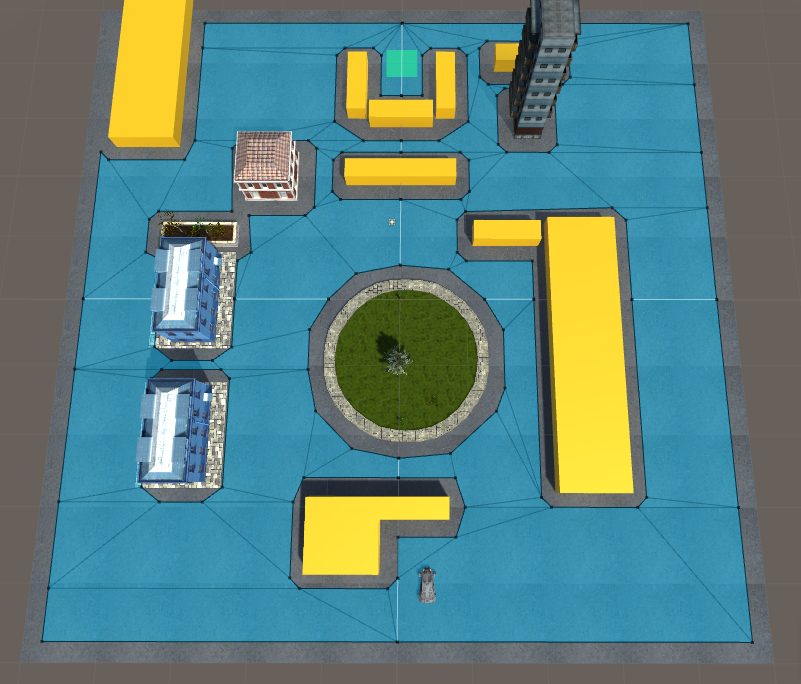
\includegraphics[width=\textwidth,height=10cm,keepaspectratio=true]{nav_mesh}
    \caption[Imagen de un \textit{Nav Mesh} en \textit{Unity}]{Imagen de un \textit{Nav Mesh} en \textit{Unity}.}
    \label{fig:basics AFM sketch}
\end{figure}

La clase \textit{NavMesh} de \textit{Unity} tiene métodos que podemos usar como \textit{RayTrace}, que lanza un rayo desde un vector a otro y devuelve si son visibles dentro de la \textit{NavMesh}, es decir, si existe una línea recta entre ellos que los una dentro del camino recorrible. Este método lo hemos usado para decidir si un nodo sucesor es válido o no. Al usarlo encontramos un \textit{bug} que producía que a veces no se encontrará el camino o bucles infinitos al recorrer las listas. Esto es debido a que puede ocurrir que no devuelva lo mismo dependiendo del orden o sentido en el que se le indiquen los vectores entre los que lanzar el rayo. Por ejemplo \textit{RayTrace}(vector1, vector2) puede ser visible pero \textit{RayTrace}(vector2, vector1) no. Para solucionarlo, tuvimos que vigilar el orden con el que recorríamos las listas, y decidimos, que cuando fuera posible, comprobar que para que fuera un sucesor válido debe ser visible en los dos sentidos.

\section{Cola de prioridad}
Uno de los problemas que se encontraron al usar C\# y en concreto la versión que utiliza \textit{Unity} ha sido el no poder usar todos las estructuras de datos de C\# y que algunas estructuras de datos no estaban disponibles directamente en C\#.

Una de estas estructuras de datos que no se encuentran en C\# es la cola de prioridad. La cola de prioridad es utilizada por el \Astar para almacenar los estados que se van a explorar. Se ordenan según su coste y se extrae de la cola aquel que tenga menos coste para ser el siguiente en ser explorado.

Para tener acceso a una cola de prioridad hemos usado
\textit{High Speed Priority Queue for C\#\cite{bluerajacola}}\footnote{\url{https://github.com/BlueRaja/High-Speed-Priority-Queue-for-C-Sharp}}.

Los motivos para utilizarla han sido que tiene una licencia MIT que permite usarla libremente. Es sencilla y fácil de usar, además está creada con el objetivo de ser usada para \textit{Path Finding} con lo que encaja en los objetivos del proyecto.

\section{Física del vehículo}
\textit{Unity} dispone de un motor de físicas integrado basado en el \textit{PhysX} de \textit{Nvidia}\footnote{\url{https://blogs.unity3d.com/es/2014/07/08/high-performance-physics-in-unity-5/}}. Una de las características que se encuentran en el motor de físicas y que han resultado de gran utilidad para la realización del proyecto han sido los \textit{Wheel Colliders}

\begin{figure}[htpb]
    \centering
    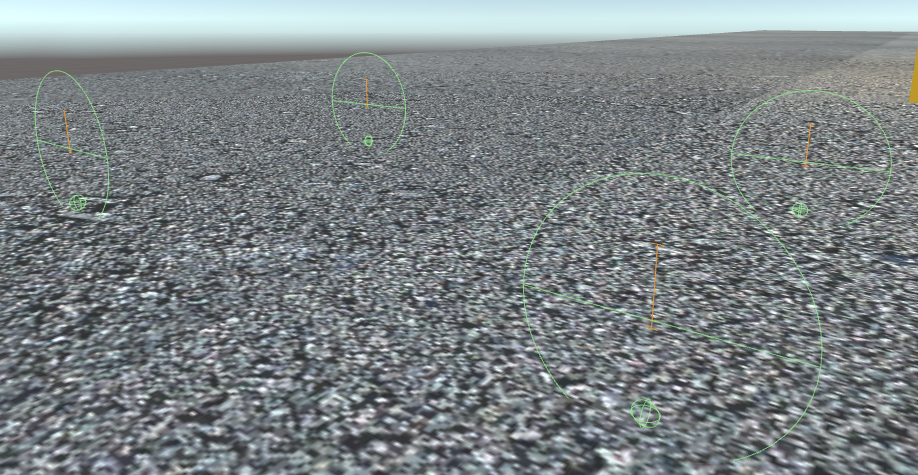
\includegraphics[width=\textwidth,height=10cm,keepaspectratio=true]{wheelcolliders}
    \caption[Representación de los \textit{Wheel Colliders} en \textit{Unity}]{Representación de los cuatro \textit{Wheel Colliders} en \textit{Unity}.}
    \label{fig:basics AFM sketch}
\end{figure}

Los \textit{Wheel Colliders} son una simulación realista de las ruedas de un vehículo y permiten simular todas la físicas necesarias para el vehículo. Tienen tanto simulación del giro de las ruedas como de la fuerza que aplica el motor a las mismas, y una simulación del freno, además de otras simulaciones como la amortiguación que no se han controlado de forma directa en este proyecto.

El uso de los \textit{Wheel Colliders} nos ha permitido la simulación realista de un vehículo con tracción a las cuatro ruedas y un radio de giro de las mismas de 45 grados. Su uso es independiente del modelo del vehículo usado, pudiendo adaptarlo a cualquier modelo cambiando sus parámetros. Tampoco hay limitaciones al número de \textit{Wheel Colliders} que podemos usar, de tal forma que es posible simular una motocicleta, un camión o cualquier otro vehículo que use ruedas.

\section{Modelos utilizados}
Los modelos usados han sido los que estaban disponibles en la \textit{Assets Store}\footnote{\url{https://www.assetstore.unity3d.com/}} de \textit{Unity}.

Principalmente hemos usado los \textit{Standard Assets 1.1.2}\footnote{\url{https://www.assetstore.unity3d.com/en/\#!/content/32351}} de \textit{Unity} de donde hemos utilizado el modelo del coche, y cuyos ejemplos nos han servido para aprender como usar \textit{Unity}.

El siguiente conjunto de \textit{assets} que más hemos utilizado ha sido \textit{Low Poly Street Pack 1.0}\footnote{\url{https://www.assetstore.unity3d.com/en/\#!/content/67475}} de \textit{Dynamic Art}, de donde hemos usado la mayor parte de los edificios y elementos del escenario.

En menor medida también se han utilizado elementos de \textit{Abandoned Building 1.0}\footnote{\url{https://www.assetstore.unity3d.com/en/\#!/content/62875}} de Aleksey Kozhemyakim, \textit{Block Building Pack 1.0}\footnote{\url{https://www.assetstore.unity3d.com/en/\#!/content/13925}} de CGY (Yemelyan K.), \textit{Building Apartment 1.0}\footnote{\url{https://www.assetstore.unity3d.com/en/\#!/content/80004}} de LowlyPoly, \textit{San Francisco House 1.0}\footnote{\url{https://www.assetstore.unity3d.com/en/\#!/content/16640}} de Bretwalda Games, \textit{UK Terraced House Pack 1.0}\footnote{\url{https://www.assetstore.unity3d.com/en/\#!/content/63481}} de rik4000.

Los \textit{assets} usados son gratuitos y siguen la licencia de la \textit{Unity Store}\footnote{\url{https://unity3d.com/es/legal/as_terms}} en el que su uso es libre dentro de juegos y de medios interactivos.

\section{Comparativa de los algoritmos}\label{comparativaAlgoritmos}

En esta sección vamos a comparar los algoritmos dependiendo de si utilizan una representación del espacio de búsqueda continua o discreta. A continuación también compararemos el rendimiento de los distintos algoritmos tomando como referencia al \Astar.

En la tabla 5.1 comparamos los algoritmos teniendo en cuenta como representan el espacio de búsqueda y que limitaciones tienen en cuenta. Podemos observar que el \textit{Hybrid \Astar} es el único que tiene en cuenta el modelo físico de los vehículos, y con ello el único que busca rutas válidas para la mayoría de los casos con vehículos no holonómicos. Además, debido a esto, es el único que puede buscar rutas que indiquen al vehículo a moverse en varios sentidos según su dirección. El resto de algoritmos realizan la búsqueda para vehículos holonómicos no teniendo en cuenta estás restricciones.

\tablaSmall{Comparación de los algoritmos según su representación}{l c c c c }{comparativadiscretocontinuo}
{ \multicolumn{1}{l}{Algoritmo} & Discreto & Continuo & Modelo Físico & Varios Sentidos \\}{ 
\Astar & X & & &\\
Theta* & X & & & \\
\Astar vértices & & X & &\\
Hybrid \Astar & & X & X & X \\
}

En la tabla 5.2 comparamos el rendimiento de los algoritmos usados en las mismas condiciones y buscando una ruta con los mismo inicio y meta. Hemos tomado el \Astar como referencia ya que el resto se basan en el. Los resultados son los esperados. El Theta* es más lento debido a los cálculos extra que debe hacer para comprobar si puede asignar un nodo anterior al nodo sucesor. La versión del \Astar con vértices es mucho más rápida debido a que el número de estados a explorar es mucho menor, al usar los vértices del \textit{Nav Mesh}. El \textit{Hybrid \Astar}, aunque es el que más cálculos debe llevar a cabo, es más rápido debido a la heurística mejorada \ref{hueristicahybrid} que le hemos incluido, donde tiene precalculado el coste desde todos los estados posibles hasta la meta teniendo en cuenta los obstáculos.

\tablaSmall{Comparación de los algoritmos según su rendimiento}{l c c }{comparativarendimiento}
{ \multicolumn{1}{l}{Algoritmo} & Segundos & Porcentaje \\}{ 
\Astar & 6.6 & 100\%\\
Theta* & 10.2 & 155.5\%\\
\Astar vértices & 2.05 & 31.1\%\\
Hybrid \Astar & 4.01 & 60.8\%\\
}

\capitulo{6}{Trabajos relacionados}

Este apartado sería parecido a un estado del arte de una tesis o tesina. En un trabajo final grado no parece obligada su presencia, aunque se puede dejar a juicio del tutor el incluir un pequeño resumen comentado de los trabajos y proyectos ya realizados en el campo del proyecto en curso. 

\capitulo{7}{Conclusiones y Líneas de trabajo futuras}

\section{Conclusiones}
En la realización de este proyecto hemos sido capaces de aprender como funciona y hemos usado un motor 3D, hemos implementado distintos tipo de algoritmos que permiten la planificación de rutas y hemos implementado métodos para el seguimiento de las mismas de forma autónoma. En general hemos sido capaces de alcanzar los objetivos que nos habíamos propuesto.

También hemos visto de primera mano las dificultades que entrañan los vehículos autónomos y nos hemos encontrado con la gran cantidad variables a considerar que no se aprecian en una primera fase cuando se están estudiando los algoritmos a usar.

Una de las mayores dificultades que hemos encontrado ha sido la planificación del proyecto, debido a que cuando empezamos no teníamos conocimiento de la mayoría de subtareas que eran necesarias para su realización, con lo que fue difícil calcular la cantidad de trabajo que llevaría cada una de ellas.

\section{Líneas de trabajo futuras}
Las posibles mejoras del proyecto son muchas, debido a que es un campo donde aún se está en desarrollo y que las disciplinas que abarca son múltiples.

Algunas de las posibilidades que planteamos son mejoras que se pueden introducir al trabajo ya realizado:
\begin{itemize}
\item Mejorar las rutas obtenidas a través de la inclusión de un mapa de Voronoi\cite{wiki:voronoi} que mejore la distancia a la que pasa el vehículo de los obstáculos. También se pueden mejorar a través de la inclusión de una heurística que precalcule la distancia a la meta teniendo en cuenta los obstáculos que hay por el camino. De este manera se puede reducir el número de estados a explorar y mejorar el rendimiento.
\item Mejorar el movimiento del vehículo usando rutas Reeds-Shepp\cite{reeds1990optimal}. Estas rutas son costosas computacionalmente pero usadas junto con el \textit{Hybrid A*} permiten mayor precisión a la hora de alcanzar la meta.
\item Crear un sistema de sensores virtuales que sea capaz de detectar el mapa en tiempo real y los obstáculos según se mueve el vehículo.
\item Añadir otros vehículos que se muevan por el mapa, creando sensores para el vehículo que sean capaces de detectar otros vehículos, su movimiento y evitar una colisión.
\item Diseñar un sistema de reconocimiento de señales de tráfico y carreteras, de tal forma que el vehículo se mueva por el carril derecho y sea capaz de respetar las señales.
\end{itemize}



\bibliographystyle{plain}
\bibliography{bibliografia}

\end{document}
